\subsection{Entwerfen von Gestaltungslösungen}

\textbf{Ziel:}
Das Ziel dieser Phase ist es, auf Basis der definierten Anforderungen und Benutzerbelange Gestaltungslösungen zu entwickeln, die den Nutzungskontext und die spezifischen Bedürfnisse der Nutzer berücksichtigen. 
Dies umfasst die Erstellung von Prototypen und die Entwicklung funktionaler \gls{browser}-Erweiterung.

\textbf{Papierprototyp:}
Ein erster Papierprototyp wurde erstellt, um die hierarchische Struktur zur Verwaltung von \gls{tab}s zu demonstrieren. Dieser Prototyp zeigt, wie Benutzer Tabs zu bestimmten Themen gruppieren und bei Bedarf auf einmal schließen können.

\begin{itemize}
    \item \textbf{Ziele des Papierprototyps:}
    \begin{itemize}
        \item Visuelle Darstellung der hierarchischen Tab-Verwaltung.
        \item Ermittlung des Benutzerfeedbacks zur intuitiven Nutzung der hierarchischen Struktur.
        \item Identifikation von Verbesserungsmöglichkeiten basierend auf dem Feedback der Nutzer.
    \end{itemize}
\end{itemize}

\begin{figure}[H]
    \caption{Papierprototyp zur Demonstration der hierarchischen Tab-Verwaltung}
    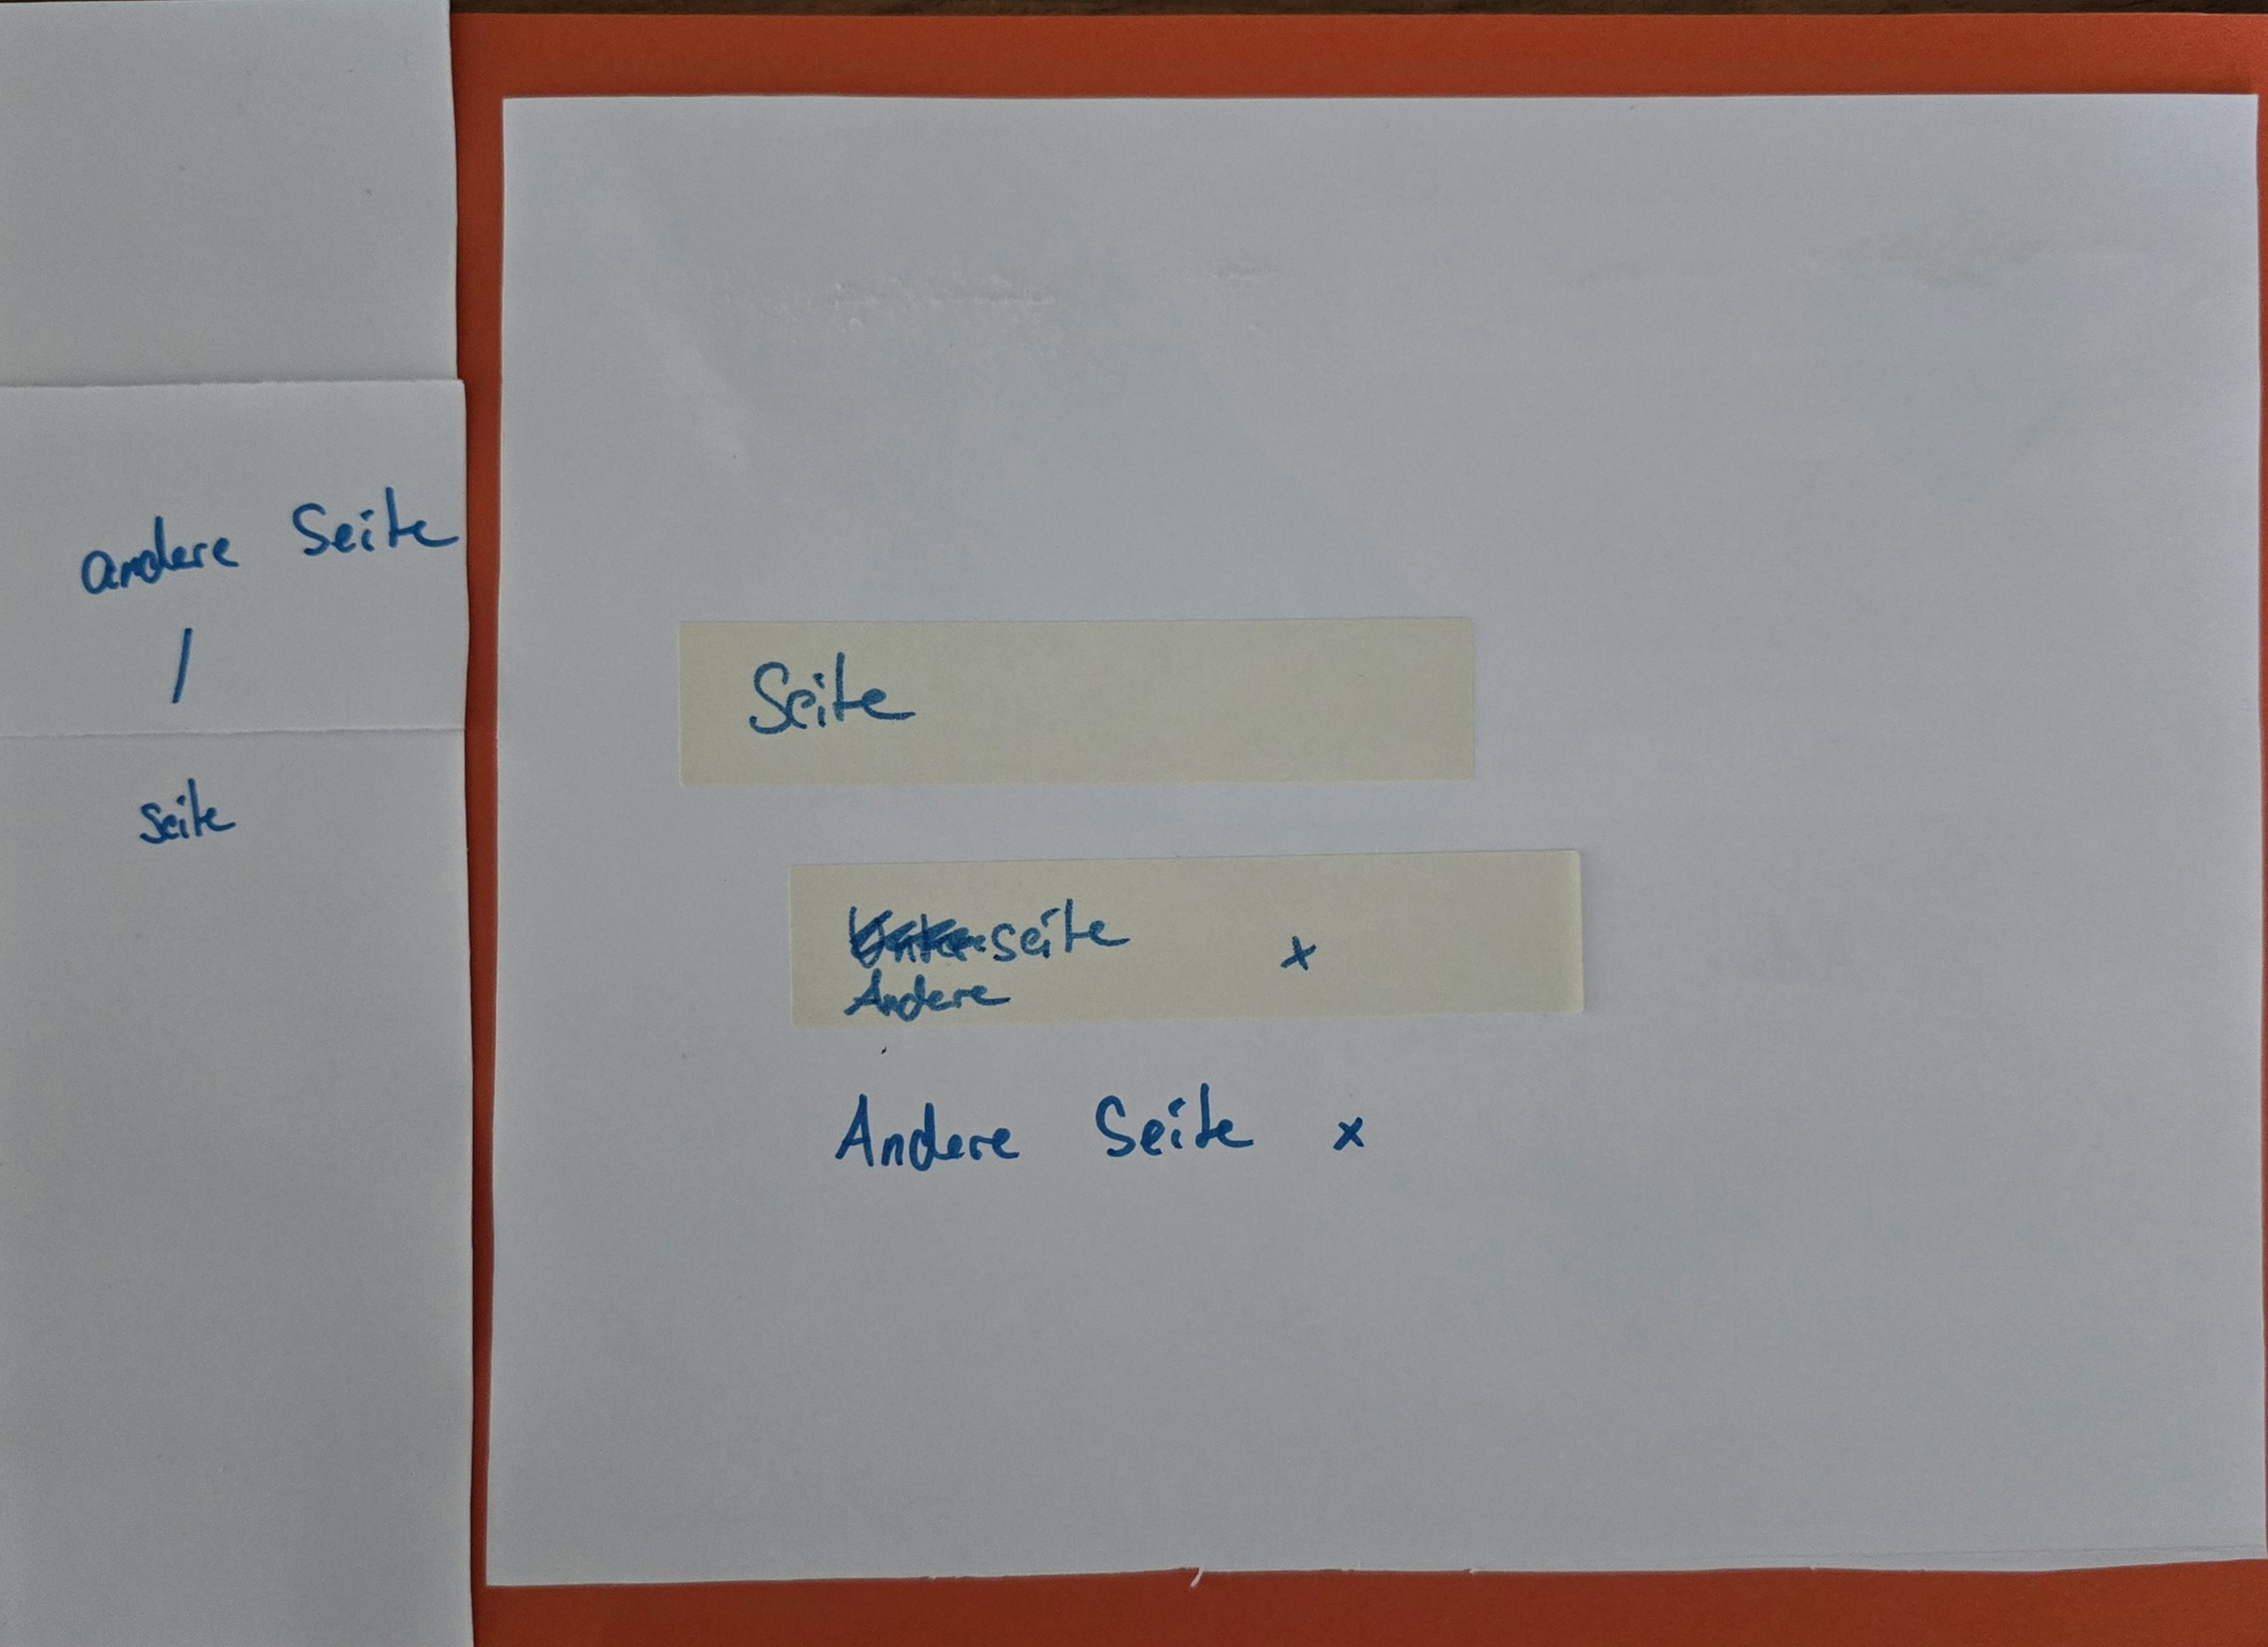
\includegraphics[height=5cm]{abbildungen/papierprototyp.jpg}
\end{figure}


\textbf{Browser-Erweiterung-Entwicklung:}
Basierend auf dem Papierprototyp wurde eine \gls{browser}-Erweiterung entwickelt, das die schnelle Navigation zwischen Tabs in der hierarchischen Struktur und das Schließen von Tabs demonstriert.

\begin{itemize}
    \item \textbf{Funktionalitäten des Plugins:}
    \begin{itemize}
        \item \textbf{Hierarchische Tab-Verwaltung:} Tabs werden auf der linken Seite basierend darauf, von welcher Seite die Tabs geöffnet wurden, zu einer bestimmten Gruppe hinzugefügt und können bei Bedarf auf einmal geschlossen werden.
        \item \textbf{Schnelle Navigation:} Benutzer können schnell zwischen verschiedenen Tabs innerhalb der hierarchischen Struktur wechseln.
    \end{itemize}
\end{itemize}

\begin{figure}[H]
    \caption{\gls{browser}-Erweiterung zur Demonstration der schnellen Navigation und Schließung von Tabs}
    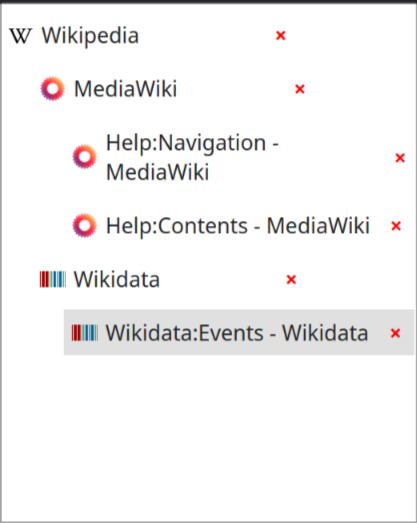
\includegraphics[height=5cm]{abbildungen/hirachie.png}
\end{figure}

\textbf{Noch zu entwickelnde Funktionalität:}
Eine Suchfunktion sowie das Verschieben der Tabs in der hierarchischen Struktur wurde bisher nicht implementiert, stellt jedoch eine zentrale Anforderung dar, die in zukünftigen Entwicklungszyklen berücksichtigt werden muss.

\begin{itemize}
    \item \textbf{Geplante Funktionalitäten:}
    \begin{itemize}
        \item \textbf{Suchfunktion:} Eine schnelle und effiziente Suchfunktion, die es ermöglicht, bestimmte \gls{tab}s schnell zu finden und zu öffnen.
        \item \textbf{Tab-Verschiebung:} Die Möglichkeit, Tabs auf einfache Weise zwischen verschiedenen Gruppen zu verschieben, um die Hierarchie anzupassen.
    \end{itemize}
\end{itemize}

\textbf{Evaluation der Gestaltungslösungen:}
Die entwickelten Prototypen und Plugins werden durch Benutzerfeedback evaluiert. Dieses Feedback wird genutzt, um die Gestaltungslösungen iterativ zu verbessern.

\begin{itemize}
    \item \textbf{Methoden zur Evaluation:}
    \begin{itemize}
        \item \textbf{Usability-Tests:} Durchführung von Usability-Tests mit echten Nutzern, um Feedback zu sammeln und die Benutzerfreundlichkeit zu evaluieren.
        \item \textbf{Feedback-Sitzungen:} Regelmäßige Sitzungen mit Stakeholdern und Nutzern, um Verbesserungsvorschläge zu diskutieren und umzusetzen.
    \end{itemize}
\end{itemize}

\textbf{Dokumentation:}
Alle Prototypen, Plugins und Evaluationsergebnisse werden detailliert dokumentiert, um den Entwicklungsprozess transparent zu gestalten und als Grundlage für zukünftige Entwicklungszyklen zu dienen.